\documentclass[conference]{IEEEtran}

\usepackage[utf8]{inputenc}
\usepackage{amsmath}
\usepackage{graphicx}
\usepackage{tabularx}
\usepackage{adjustbox}
%\usepackage[colorinlistoftodos]{todonotes}
\usepackage{csquotes}
\usepackage{comment}
\usepackage{imakeidx}
%tabela
\usepackage{multirow}
\usepackage{xcolor}
\usepackage[margin=2.5cm]{geometry}
\usepackage{hyperref} %to show links
\usepackage{titling}
\usepackage[ddmmyyyy]{datetime}
\usepackage{setspace}
\usepackage{indentfirst}

%to define placement of tables and images in strict mode
%\usepackage{placeins}

\usepackage[style=ieee]{biblatex} 
\addbibresource{ref.bib}
\input{vars}
\linespread{1.2}

\bibliography{sources}

\begin{document}

\title{Implementing an HTML5 mobile simulation utilizing web workers}

\author{authored by\\
        Lari Alakukku (528362),
        Miika Rouvinen (356770),
        Ilkka Malassu (430463)}%

\makeatletter         
\def\@maketitle{
\begin{center}
{\Huge \bfseries \sffamily \@title }\\[4ex] 
Submitted on \@date\\
{\normalsize \@author}\\[4ex] 
%\@date\\[8ex]
\end{center}}
\makeatother


% make the title area
\maketitle

\begin{IEEEkeywords}
HTML5, web, workers
\end{IEEEkeywords}

%%%%%%%%%%%%%%%%%%%%%%%%%%%%%%%%%%%%%%%%%%%%%%%%%%%%%  
\begin{abstract}

HTML5 introduced web workers as a way to utilize concurrent computation in the domain of web-based JavaScript applications. This opened up the possibility to host 
computationally demanding applications with the web browser while attempting to maintain a high quality of experience.

This paper follows the implementation of a computer physics simulation and compares the architectural decisions that can be applied to it. Different architectures with and 
without web workers are analysed and compared in terms of their performance metrics such as FPS, memory usage, processing delay and message transfer time. The perceived 
quality of the simulation is also compared between the different versions.
 
\end{abstract}

\section{Introduction}
\label{chap:introduction}

The internet has progressed from a distributed document sharing system to a platform that can host computationally demanding applications. This evolution makes performance a crucial web-client requirement. The modern browser provides a possibility to develop intricate web applications utilizing only HTML, CSS and JavaScript. However, the developers of a web-based game, for example, need to optimize their code taking the processing capability of different browsers into account. Current hardware mostly focuses on concurrent execution while many web applications still only use the main browser thread for all the computation tasks. HTML5 introduced web workers as a first step towards concurrent execution in web applications. \cite{doha}

Web workers operate by offloading processing tasks from the main browser thread to background worker threads, requiring the platform to have basic support for concurrency. 
The communication between the threads is facilitated with message sending. The process of main thread web worker communication is illustrated in Figure \ref{fig:figure1}. 
The main thread uses the "postMessage" function to send a message to a worker thread. The worker thread can handle this message using the "onMessage" function. The parameters x and y of Figure \ref{fig:figure1} represent the data, that can be shared via the messaging interface. \cite{doha, watanabe}

Web workers also have some limitations. They can not use DOM operations or access window objects and parent objects. Also, direct data sharing between the main thread and 
the worker threads is not possible. JavaScript is also unable to access the underlying hardware information of a computer to, for example, fetch the number of CPU cores. \cite{watanabe, verdu}

This paper follows and compares the architecturally different implementations of a computer physics simulation. These architectures apply different ways to implement a 
web-based application with and without web workers. The comparison is done with respect to performance metrics such as FPS, memory usage, message transfer time, processing delay and 
perceived quality. After this introduction, section \ref{sec:soa} of this paper covers the literature and studies related to web workers. Section \ref{sec:implementation} describes all the
physics simulation implementations made for the purposes of this research paper. Section \ref{sec:sec2} evaluates and compares the performance of these implementations and
Section \ref{sec:conc} concludes this paper.

\begin{figure}[ht]
	\centering
	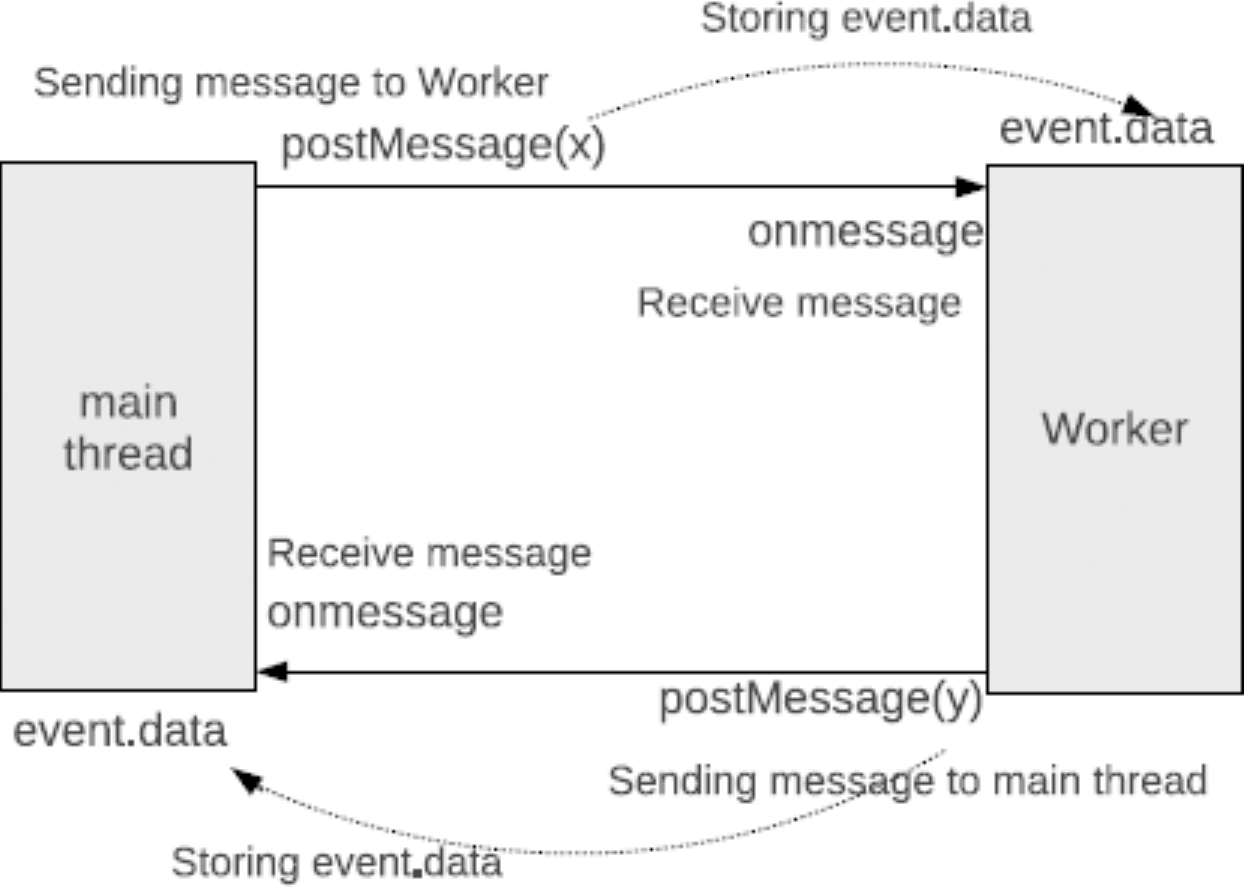
\includegraphics[scale=0.25]{figs/figure1.png}
	\caption{Communication between the main thread and worker threads \cite{watanabe}.}
	\label{fig:figure1}
\end{figure}

\section{Related Work}
\label{sec:soa}

For web-based games, Erbad et al. \cite{doha} propose a concurrent processing solution called DOHA, which aims to provide better control over quality by unlocking the 
multi-core processing capabilities. This solution consists of game event-loops running in worker threads and MultiProc, which is the module for scheduling, state 
management and other concurrent execution related tasks. Their game implementation had three main components: simulation, graphics rendering and AI. The main thread 
handles rendering and offloads game event processing to web workers. This communication also requires the sending of state information. In general, DOHA offered better 
scalability and responsiveness across different platforms. However, thread communication required replicating state across workers, which increased jitter.

Zhang et al. \cite{zhang} introduce WWOF, which is a framework for seamlessly offloading web workers to the cloud. Their study investigated applying the framework to an 
interactive animation application with a substantial amount of animation events and moving objects rendered on the screen. The main thread of the application would send 
state data to the worker threads, which would then, after sending and receiving an acknowledgement message proceed to update this data according to the simulation rules. 
All this data would then be sent back to the main thread for merging and rendering. On average, the framework achieved energy savings of 85\% on devices such as mobile 
phones, desktop computers and pads. The performance of the devices improved by a factor of 2-4.

Verdú et al. \cite{verdu} examine how utilizing web workers scales the performance of a JavaScript application. Their research investigated using varying amounts of 
workers in a synchronous ray tracing application and in an asynchronous hash calculation task. They found that the optimal number of workers depends on various factors 
such as the CPU architecture, the worker execution model and the browser. Using a large number of web workers did not prove to be beneficial compared to using only a few.

\section{Implementation}
\label{sec:implementation}

This section covers the different architectures of the physics simulation application implemented in this paper. The main idea of the simulation is to generate a given amount
of spherical objects and simulate their interactions via a graphical interface. These objects have attributes such as position, radius, velocity and acceleration. The 
physics of the application includes simulating explosions and collisions between the objects. The number of these objects is changed to investigate the behaviour
of the different architectures of the simulation.

Figure \ref{fig:figure2} shows the default user interface of the application running the simulation.

\begin{figure}[ht]
	\centering
	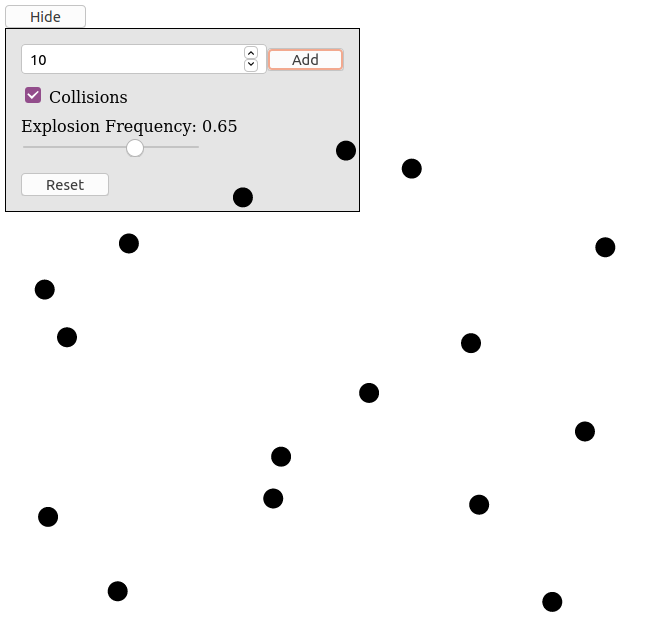
\includegraphics[scale=0.5]{figs/figure2.png}
	\caption{User interface of the simulation application.}
	\label{fig:figure2}
\end{figure}

\subsection{Default simulation} 
\label{sec:default}

The first implementation of the physics simulation only utilized the main DOM thread in computation. This default architecture of the application implemented classes for the
spherical objects, their interactions and the physics stage. A class utilizing the PIXI JavaScript library was implemented for managing the game loop, rendering and
physics simulation objects.

\subsection{Spatial partitioning} 
\label{sec:spatial}

The first architectural decision only optimized the simulation by partitioning the physics space and it did not yet include web workers. This implementation added a grid object used in constructing the physics space in a tree data structure.

\subsection{One worker solution} 
\label{sec:1workers}

After the spatial partitioning solution, an implementation with a single web worker communicating with the main thread was made. This version initialized the objects used
in physics simulation only in the worker thread. The worker thread executed the simulation and communicated the state information to the main thread via the messaging 
interface. The only responsibility of the main thread was then to read the received information and render the graphics accordingly.

\subsection{Multiple workers solution} 
\label{sec:nworkers}

After re-factoring the application architecture to support calculating the simulation steps in a worker thread, the number of web workers was increased. In this solution,
the main DOM thread communicated with a worker planner class, that organized and divided the computational tasks to be passed to multiple workers. After all the worker
threads have finished calculating their respective simulation steps, the changes to the data have to be assembled, merged and rendered in the main thread.

\subsection{Data sharing}

As stated in Section \ref{chap:introduction}, web workers communicate with the main thread and other threads via message sending. If data needs to be passed from one thread
to another, this data needs to be serialized to JSON. This paper also investigates how message sending affects the performance of the simulation by implementing a version
where the data is shared using a SharedArrayBuffer JavaScript object. This tool only supports sharing the data in a binary format, but it makes the data accessible from all the worker threads.

\section{Methods}
\label{sec:methods}

This section describes the methods used for evaluating the different architectures of the simulation application implemented for the purposes of this paper. The metrics used for evaluating it's performance are FPS, memory usage, message transfer time, processing delay and changes in user experience.

\subsection{Developer tools}

Browsers such like Firefox and Chrome offer a possibility to more closely inspect web services through developer tools. These tools offer insights into how demanding a given application
is on the computational resources accessible by the browser. Memory usage and the FPS (frames per second) values given by developer tools are evaluated in the simulation
case of this paper.

\subsection{Timestamps}

JavaScript timestamp functionality provides a possibility log timestamps to the console from different stages of application execution. This paper uses these timestamps to
measure the processing delays caused by updating the simulation state in the cases of different architectures.

\subsection{Perceived quality}

The perceived quality of the simulation implementations is also measured by observing the executing application user interface visually. These implementations are compared
with respect to the amount of visually prominent jitter they produce. Any other deviations in user experience between the simulation versions are also investigated.

\section{Evaluation}
\label{sec:sec2}

Here we present our evaluation of the implementation.

\section{Conclusions}
\label{sec:conc}

We conclude our research paper here.

\printbibliography[title={References}]

\end{document}